\chapter{Конструкция недеформируемого водного робота с острой кромкой}\label{ch:ch5}

В данной главе описана конструкция недеформируемого водного робота с острой кромкой. Представлена кинематическая схема, описаны основные элементы конструкции. Представлен состав системы управления, и описаны ее основные элементы.

Для возможности сравнения результатов размеры и массо-геометрические характеристики робота приближены к роботу, описанному в работе~\cite{Pollard_Tallapragada_2016}.

\section{Описание конструкции недеформируемого водного робота с острой кромкой}

Робот представляет собой полый объект, в продольном сечении имеющий форму профиля крыла NACA 0040 (см. рисунок \ref{Photo_NACA}) длиной 340 мм, шириной 134 мм. Высота робота 80 мм. Форма профиля крыла NACA 0040 задается функцией 
$ y = \frac{T}{0.2}(a_0\sqrt{x} + a_1x + a_2x^2 + a_3x^3 + a_4x^4 $, где $a_0=0.2969$, $a_1=-0.126$, $a_2=-0.3516$, $a_3=0.2843$, $a_4=-0.1036$, $T=0.4$. Точки контура профиля были рассчитаны в среде Matlab и импортированы в среду разработки Компас-3Д.	

\begin{figure}[h]
	\centering
	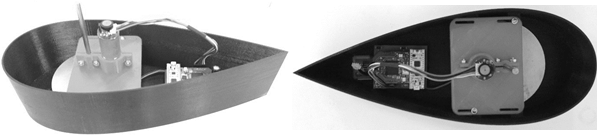
\includegraphics[width=1\linewidth]{Photo_NACA.png}%
	\caption{Недеформируемый водный робот с острой кромкой}
	\label{Photo_NACA}
\end{figure}

\begin{figure}[h]
	\centering
	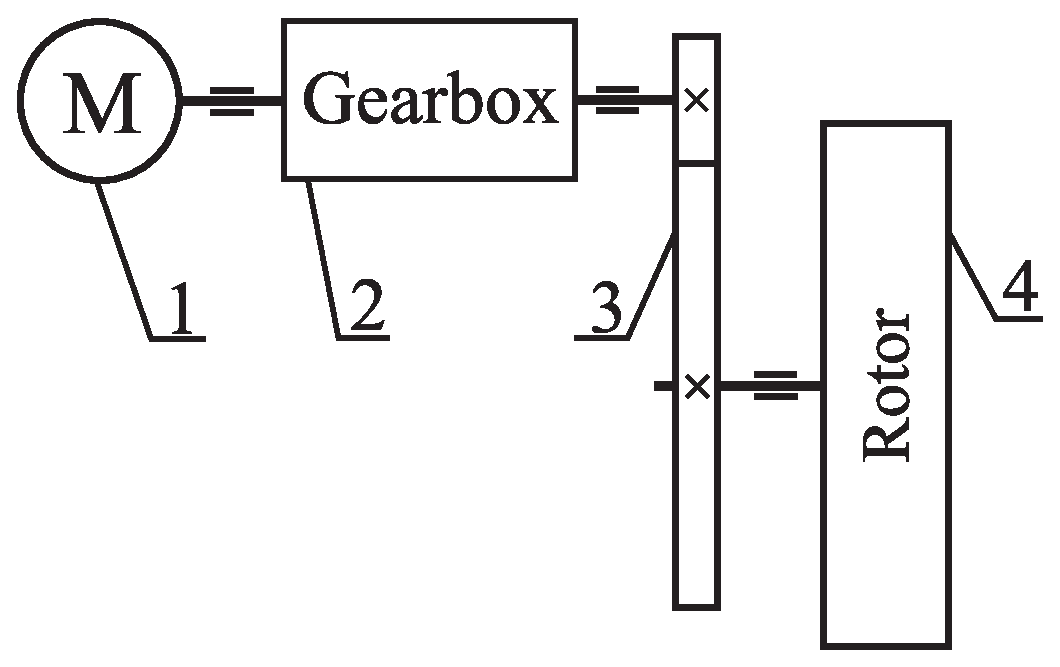
\includegraphics[width=0.5\linewidth]{Kinematic_Scheme2.eps}%
	\caption{Кинематическаая схема передачи вращения от двигателя к ротору}
	\label{kinemSchemeNACA}
\end{figure}

Корпус изготовлен на 3Д-принтере из PLA-пластика с толщиной стенки в 2 мм. Внутри корпуса закреплен ротор 4 с двигателем 1 таким образом, что центр масс всей системы находится максимально близко к нижней грани робота. Для передачи вращения с двигателя к ротору использовалась пара шестерен 3 с передаточным отношением 3.5:1. Кинематическая схема передачи вращения от двигателя к ротору представлена на рисунке~\ref{kinemSchemeNACA}.



Внутри также располагается элемент питания и плата с микроконтроллером модели STM32F303K8T6, управляющим вращением двигателя постоянного тока. 

В качестве модуля питания используется литий-полимерная (Li-Po) аккумуляторная батарея фирмы nVision с номинальным напряжением 7.4 Вольт, емкостью 450 мАЧ и максимальным выходным током до 13.5 Ампер.


Микроконтроллер расположен на отладочной плате Nucleo-32 от фирмы STMicroelectronics. Данная плата имеет 30 выводов; содержит программатор ST-Link, с помощью которого можно программировать микроконтроллер, подключив плату к персональному компьютеру по USB-кабелю; имеет необходимую обвязку из электронных компонентов, необходимых для стабильной работы микроконтроллера, кнопку сброса микроконтроллера и 3 светодиода: один пользовательский светодиод, светодиод, отображающий подачу питания на плату, и светодиод, сигнализирующий о передаче данных по USB-интерфейсу; может питаться как от USB-кабеля, так и от внешнего напряжения 7--15 Вольт. Данная плата поддерживает среду разработки ARM mbed, которая позволяет разрабатывать программное обеспечение для микроконтроллера, используя онлайн среду программирования. Внешний вид отладочной платы Nucleo-32 представлен на рисунке~\ref{Nucleo}. Характеристики микроконтроллера STM32F303K8T6 представлены в таблице~\ref{tabStm}.

\begin{figure}[h]
	\centering
	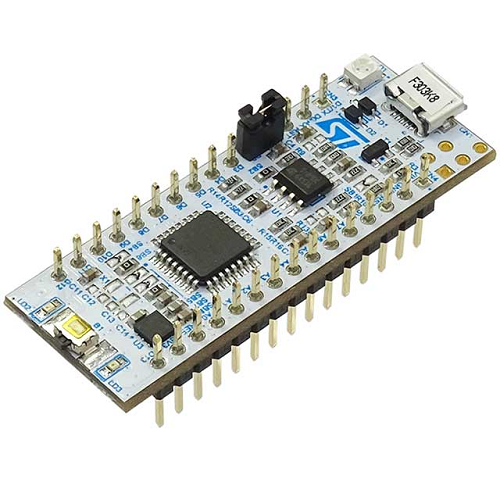
\includegraphics[width=0.4\linewidth]{Nucleo.png}%
	\caption{Отладочная плата Nucleo-32 с микроконтроллером STM32F303K8T6}
	\label{Nucleo}
\end{figure}

\begin{table}[h]
	\centering
	\caption{Характеристики микроконтроллера STM32F303K8T6}\label{tabStm}
	\begin{tabular}{|l|c|}
		\hline
		Производитель &	STMicroelectronics (ST) \\ \hline
		Корпус 	& LQFP \\ \hline
		Тмакс	&	85$^\circ$ C 	\\ \hline
		Тмин 	&	-40$^\circ$ C \\ \hline
		Оперативная память 	& 16 КБайт\\ \hline
		Тактовая частота	& 72 МГц 	\\ \hline
		Flash память & 64 КБайт\\ \hline
		Архитектура ядра & Cortex-M4	\\ \hline
		Кол-во выводов 	& 32\\ \hline
		Разрядность	& 32 бита\\ \hline
		Количество входов / выходов & 25	\\ \hline
		Интерфейсы 	& CAN, I2C, SPI, USART\\ \hline
		Разрешение АЦП & 12 бит\\ \hline
		Диапазон напряжений питания 	& 2...3.6 Вольт\\ \hline		
	\end{tabular}
\end{table}


Для управления двигателем постоянного тока также используется драйвер VNH3SP30 фирмы STMicroelectronics, описанный в главе~\ref{ch:ch3}. Характеристики данного драйвера представлены в таблице~\ref{tabVnh}. Для работы с недеформируемым водным роботом с острой кромкой используется модуль на базе драйвера VNH3SP30 (см. рисунок~\ref{DriverPcb}). 


В качестве двигателя использовался мотор-редуктор с энкодером. Характеристики двигателя представлены в таблице~\ref{tabMotor2}. 

\begin{table}[h]
	\centering
	\caption{Характеристики двигателя}\label{tabMotor2}
	\begin{tabular}{|l|c|}
		\hline
		Номинальное напряжение питания & 6 В \\ \hline
		Передаточное отношение редуктора & 34:1 \\ \hline
		Момент на валу & 0.64 Нм\\ \hline
		Максимальная скорость вращения & 280 об/мин \\ \hline
		Ток холостого хода & 550 мА\\ \hline
		Пусковой ток & 6.5 А \\ \hline
	\end{tabular}
\end{table}


Энкодер, расположенный на валу двигателя, использовался для определения положения ротора в течение экспериментов. Данный энкодер имеет специальный магнитный диск и датчики Холла, с помощью которых формируются сигнальные импульсы. Энкодер имеет два канала со смещением сигнала в четверть периода относительно друг друга, что позволяет определять направление вращения вала двигателя. Каждый канал формирует 12 импульсов на один оборот вала двигателя. Таким образом, используя два канала, считая переходы сигнала от низкого уровня к высокому и от высокого к низкому, можно получить 48 импульсов на один оборот вала двигателя. На микроконтроллере данные с энкодера обрабатываются таймером TIM1, который имеет специальный режим работы с энкодером (Encoder Mode), что позволяет аппаратно считать количество импульсов с двух каналов, учитывая направление вращения. 

Дифференцируя данные, полученные с энкодера, можно получить угловую скорость и угловое ускорение ротора.






Реальная модель робота имеет следующие характеристики: m = $0.905$ кг; $I_0$ = $0.00844$ кг$\cdot$м2; Ротор изготовлен из алюминия, имеет внешний диаметр 110 мм, высоту 12 мм. Масса ротора $m_r$ = $0.327$ кг; момент инерции ротора $I_r$ = $0.00058$ кг$\cdot$м2. Конструкция робота позволяет смещать центр вращения ротора.

Управление осуществляется с персонального компьютера, для которого было разработано специальное программное обеспечение. Все команды роботу передаются по беспроводному каналу связи, используя Bluetooth.


\section{Описание системы управления недеформируемого водного робота с острой кромкой}

Для управления недеформируемым водным роботом с острой кромкой была разработана система управления, структурная схема которой представлена на рисунке~\ref{ControlSystem}.

\begin{figure}[!h]
	\centering
	\includegraphics[width=0.8\linewidth]{ControlSystem.eps}
	\caption{Структурная схема системы управления недеформируемого водного робота с острой кромкой}
	\label{ControlSystem}
\end{figure}

На схеме $ \omega_{set} $ -- заданная скорость вращения ротора. Блок регулятора скорости представляет собой ПИД-регулятор, который обеспечивает поддержание значения заданной скорости $ \omega_{set} $. На выходе данного блока получаем ШИМ-сигнал необходимой скважности. Коэффициенты ПИД-регулятора подобраны экспериментально. Далее ШИМ-сигнал подается на драйвер двигателя постоянного тока, который его усиливает до необходимого напряжения и подает на обмотки двигателя. В данной работе используется драйвер двигателя постоянного тока VNH3SP30 фирмы STMicroelectronics. На валу двигателя располагается датчик положения вала (инкрементальный энкодер с 48 импульсами на оборот), с помощью которого измеряется угол поворота вала двигателя $ \varphi $. Далее с помощью блока расчета угловой скорости ротора, учитывая передаточные отношения редуктора и шестерен, получаем значение $ \hat{\omega}_{set} $ -- фактическую скорость вращения ротора. Полученное значение $ \hat{\omega}_{set} $ учитывается блоком регулятора скорости при расчете управляющих сигналов, идущих на двигатель. При вращении ротора данный алгоритм должен выполняться через промежутки времени $ \Delta t \rightarrow 0 $. Выбранный микроконтроллер имеет максимальную частоту работы 72 МГц, что позволяет выбрать $ \Delta t = 1 $ мс. Значение $ \Delta t $ выбрано экспериментально.

Для реализации управляемого движения недеформируемого водного робота с острой кромкой было разработано программное обеспечение нижнего и верхнего уровня.

В программе нижнего уровня реализованы функции управления двигателем, на котором закреплен ротор: движение по прямой и движение по некоторому радиусу. Программа принимает и обрабатывает команды с верхнего уровня (персональный компьютер, планшет, смартфон) по беспроводному каналу связи Bluetooth. Bluetooth-модуль расположен на плате системы управления и соединен с интерфейсом USART микроконтроллера. Командами задаются значения угловой скорости ротора, время вращения ротора на заданной скорости и время перехода от одной скорости вращения к другой. Реализованы команды начала вращения ротора по установленным параметрам и его остановки.

На двигателе установлен датчик углового перемещения вала – энкодер. Программа считывает с него данные, рассчитывает текущее положение ротора, учитывая передаточное отношение редуктора, и сохраняет эти данные в памяти микроконтроллера. По запросу эти данные отправляются на программное обеспечение верхнего уровня. Также с помощью численного дифференцирования можно получить фактическую угловую скорость и угловое ускорение ротора. Значение фактической угловой скорости используется в программе для поддержания заданной скорости вращения ротора.

Программа нижнего уровня предназначена для отладочной платы Nucleo-32, на борту которой расположен микроконтроллер STM32F303K8T6. Это 32-разрядный микроконтроллер с ядром ARM Cortex-M4, работающий на частоте до 72 МГц.

Программа верхнего уровня разработана для смартфона на операционной системе Android версии не ниже 9 с помощью онлайн-сервиса MIT App Inventor. В данном сервисе используется визуальный язык программирования, который позволяет разработать приложение, используя графический интерфейс. Интерфейс программы представлен на рисунке~\ref{AndroidScreen}.

%\begin{figure}[!h]
%	\centering
%	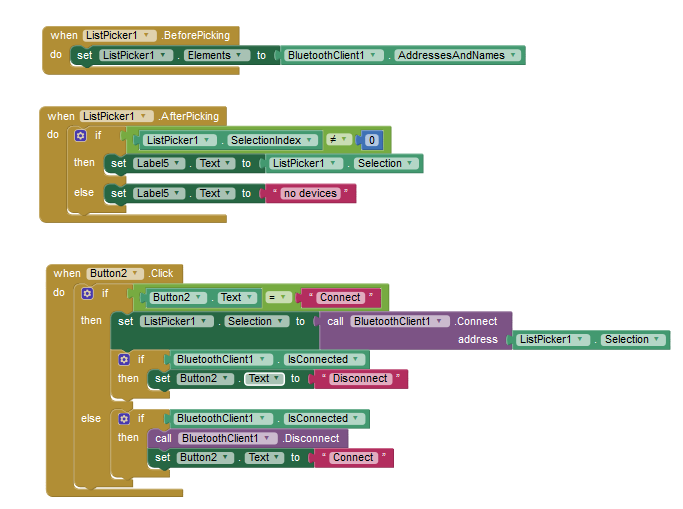
\includegraphics[width=0.7\linewidth]{AndroidInventor.png}
%	\caption{Разработка андроид-приложения в MIT App Inventor}
%	\label{AndroidInventor}
%\end{figure}

%Интерфейс программы представлен на рисунке~\ref{AndroidScreen}.

\begin{figure}[!h]
	\centering
	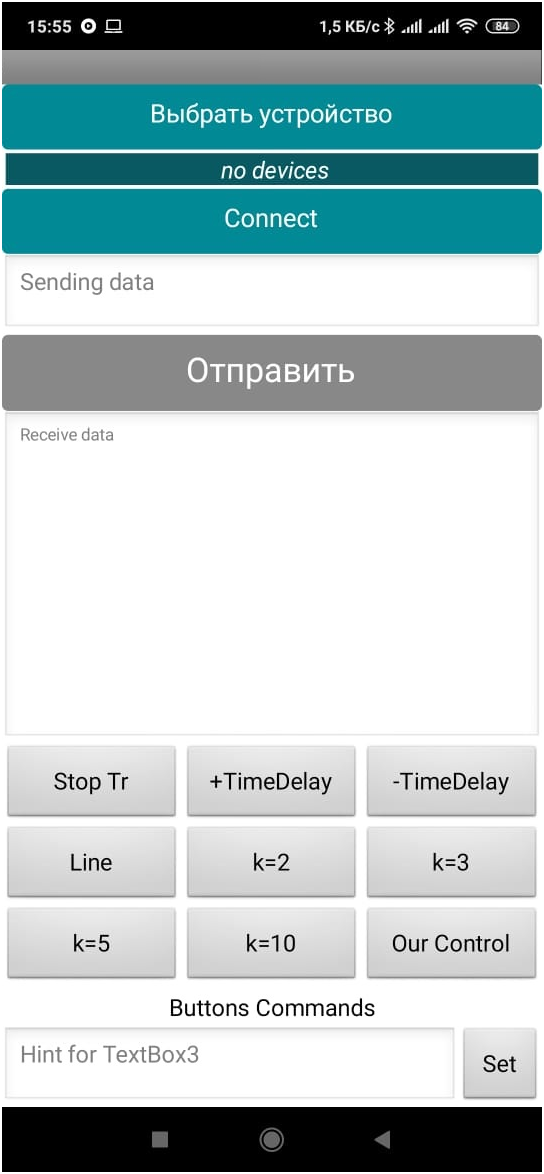
\includegraphics[width=0.3\linewidth]{AndroidScreen.png}
	\caption{Интерфейс программы управления безвинтовым недеформируемым рыбоподобным надводным роботом}
	\label{AndroidScreen}
\end{figure}

Данная программа позволяет подключится к bluetooth-устройству, установленному на роботе, передавать и принимать необходимые команды. Используя поле <<Sending data>>, можно отправить необходимую последовательность байтов роботу. В поле <<Receive data>> отображаются данные, принятые от робота. Программа позволяет управлять роботом, используя разные режимы движения: запуск и остановка вращения ротора для движения по прямой и по окружности, изменение периода управляющих импульсов.

%Длительное нажатие на кнопку позволяет изменить команду, присвоенную кнопке при помощи поля "Buttons Commands".

%\section{Отладка системы управления}
%
%\qquad После монтажа элементов на печатную плату системы управления, были проверены цепи питания и "земли" на короткое замыкание. После успешной проверки плата подключалась к блоку питания для мониторинга потребляемого тока. Рабочий ток платы на холостом ходу не должен превышать 50 мА.
%
%После загрузки прошивки в микроконтроллер был проверен канал связи. В режиме отладки необходимо убедиться, что все команды, отправляемые с программы верхнего уровня, доходят без ошибок до программы нижнего уровня; данные с программы нижнего уровня доходят без ошибок до программы верхнего уровня.
%
%После успешной проверки можно установить плату системы управления в корпус робота, подключить двигатель и аккумулятор и еще раз проверить все команды с подключенным двигателем и вращением ротора.


\clearpage